\section{Random-walk correlation: full results}
\label{sec:appendix-corr}

Figure~\ref{fig:corr-matrices} shows ground-truth and predicted $4\times4$
correlation matrices for a random selection of test samples.

\begin{figure}[H]
  \centering
  
\includegraphics[width=\linewidth]{figures/corr_matrix_heatmaps.png}
  \caption{Predicted (left half) vs.\ true (right half) correlation
    matrices for six test samples drawn from the 800-sample test set.}
  \label{fig:corr-matrices}
\end{figure}

Figure~\ref{fig:corr-baselines} compares the recovery head against two
analytic baselines computed directly from the observed series: the
Pearson correlation of the raw values (\emph{position corrcoef}, a
naive but often-used estimator) and the Pearson correlation of
first differences $\Delta x_t$ (\emph{diff corrcoef}, the
maximum-likelihood estimator for this model).  The head sits near the
diff-corrcoef ceiling and well above the position-corrcoef baseline
($r\approx 0.50$), which demonstrates that the backbone is not merely
exploiting the spurious correlations that accumulate in random-walk
levels.

\begin{figure}[H]
  \centering
  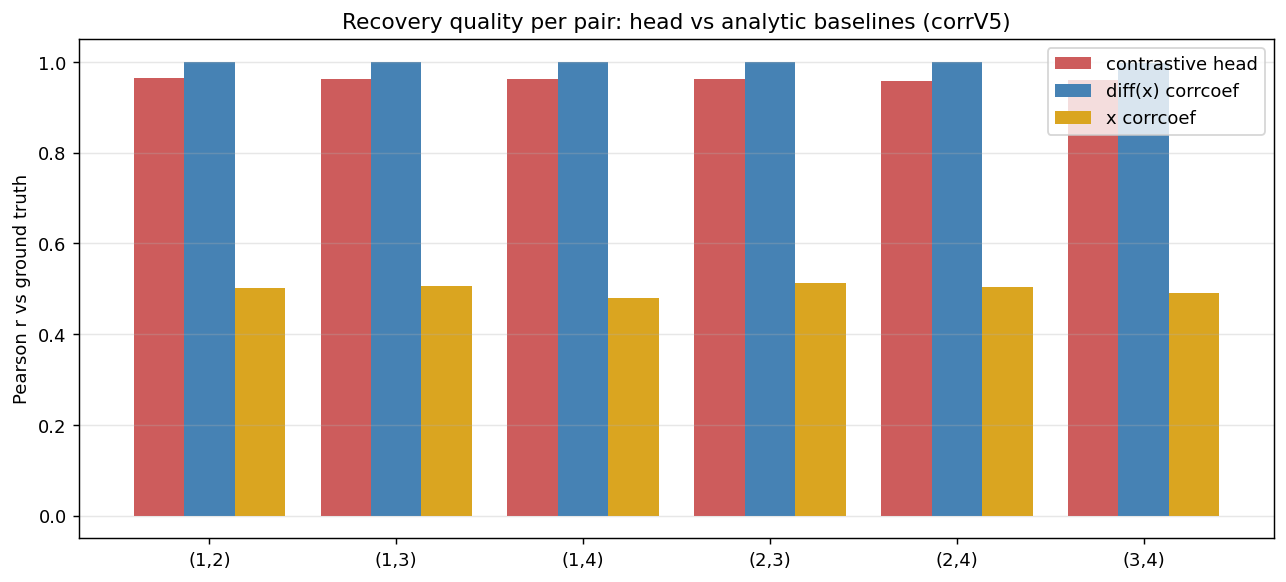
\includegraphics[width=0.75\linewidth]{figures/corr_baseline_comparison.png}
  \caption{Per-pair Pearson $r$ for the recovery head (blue), the
    diff-corrcoef analytic ceiling (red), and the position-corrcoef
    baseline (yellow).}
  \label{fig:corr-baselines}
\end{figure}

Figure~\ref{fig:corr-errors} shows the per-sample MSE distribution on
the 800-sample test set.

\begin{figure}[H]
  \centering
  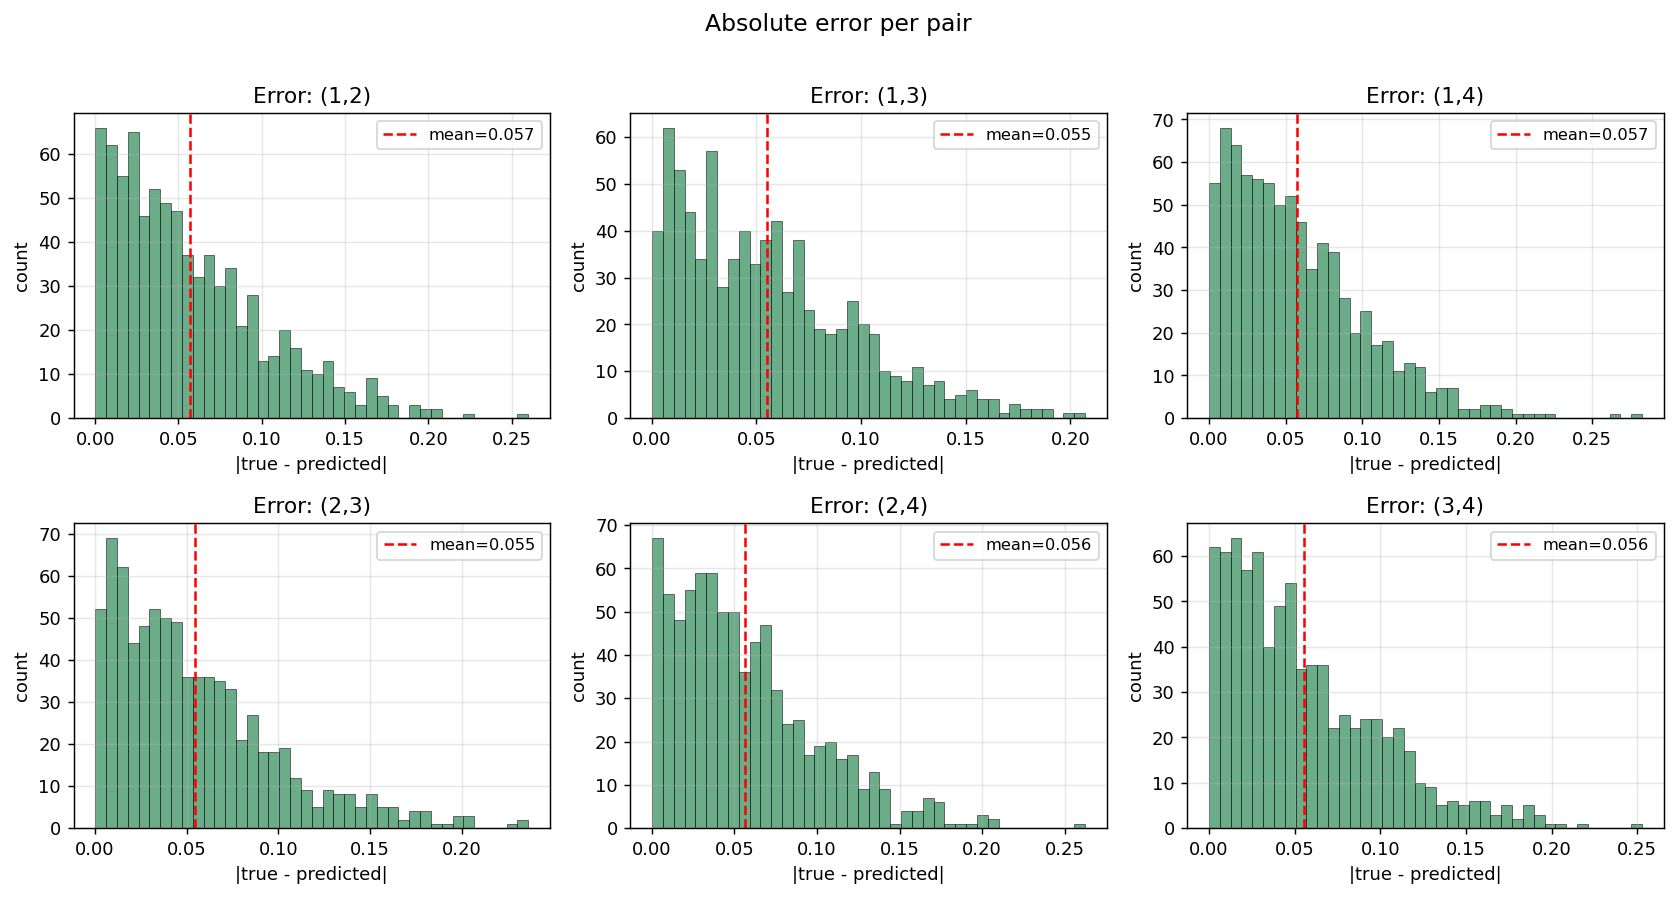
\includegraphics[width=0.65\linewidth]{figures/corr_error_distributions.png}
  \caption{Per-sample MSE distribution for the correlation recovery head
    on the 800-sample test set.}
  \label{fig:corr-errors}
\end{figure}
